\documentclass[tikz,border=8pt]{standalone}
\usepackage[T1]{fontenc}\usepackage{lmodern,amsmath,amssymb}\usetikzlibrary{arrows.meta,positioning,fit}
\begin{document}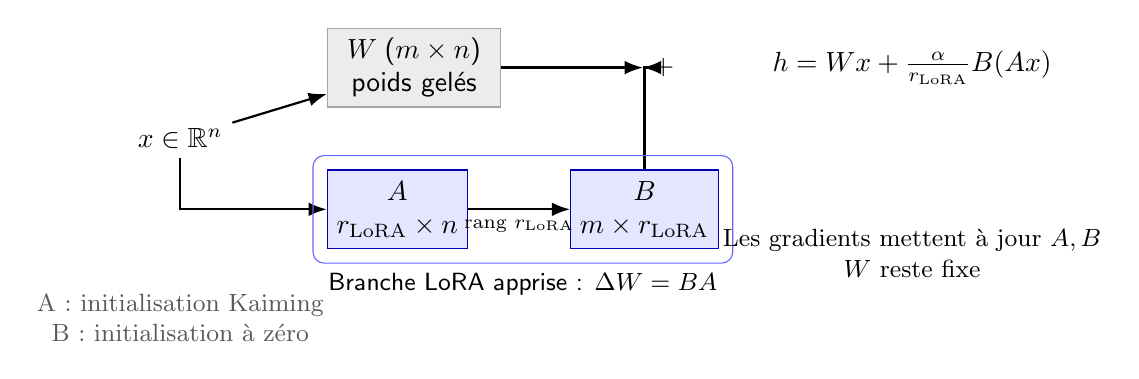
\begin{tikzpicture}[font=\sffamily,>=Latex,fixed/.style={draw=gray!70,fill=gray!15,minimum width=2.2cm,minimum height=1cm,align=center},train/.style={draw=blue!70!black,fill=blue!10,minimum width=1.7cm,minimum height=1cm,align=center},arr/.style={-{Latex},thick}]
\node (x) {$x\in\mathbb R^n$};
\node[fixed,right=12mm of x,yshift=9mm] (W) {$W$\;($m\times n$)\\poids gelés};
\node[train,right=12mm of x,yshift=-9mm] (A) {$A$\\$r_{\rm LoRA}\times n$};
\node[train,right=13mm of A] (B) {$B$\\$m\times r_{\rm LoRA}$};
\node[right=18mm of W] (sum) {$+$};\node[right=10mm of sum] (h) {$h=Wx+\frac{\alpha}{r_{\rm LoRA}}B(Ax)$};
\draw[arr] (x)--(W);\draw[arr] (W)--(sum);\draw[arr] (x)|-(A);\draw[arr] (A)--node[below,font=\scriptsize]{rang $r_{\rm LoRA}$}(B);\draw[arr] (B)|-(sum);
\node[draw=blue!60,rounded corners,fit=(A)(B),inner sep=5pt,label=below:{\small Branche LoRA apprise : $\Delta W=BA$}] {};
\node[below=16mm of x,align=center,font=\small,text=gray!70!black] {A : initialisation Kaiming\\B : initialisation à zéro};
\node[below=16mm of h,align=center,font=\small] {Les gradients mettent à jour $A,B$\\$W$ reste fixe};
\end{tikzpicture}\end{document}
